
% Vuforia is a software platform that enables the creation of \ac{ar} experiences. 
% % Integrated with Unity, a leading platform for developing games and interactive applications, Vuforia simplifies the incorporation 
% of AR into mobile and digital apps. 
% It uses computer vision technologies to recognize and track images and objects in the real world, allowing developers to overlay digital 
% content precisely.

% The marker illustrated in Figure \ref{f:aruco_marker} was selected following initial attempts that yielded inconsistent results when using 
% the laptop's camera, shown in the figure \ref{fig:camera-c922}, to scan the environment. This particular marker demonstrated greater stability, 
% enabling the precise positioning of the digital UR10 model in alignment with the physical surroundings. Consequently, this facilitated the accurate 
% overlay of the digital UR10 model onto the actual UR10e robot, enhancing the integration of virtual and real-world elements.

% \begin{figure}[h]
%     \centering
%       \begin{subfigure}[b]{0.45\textwidth}
%       \centering
%       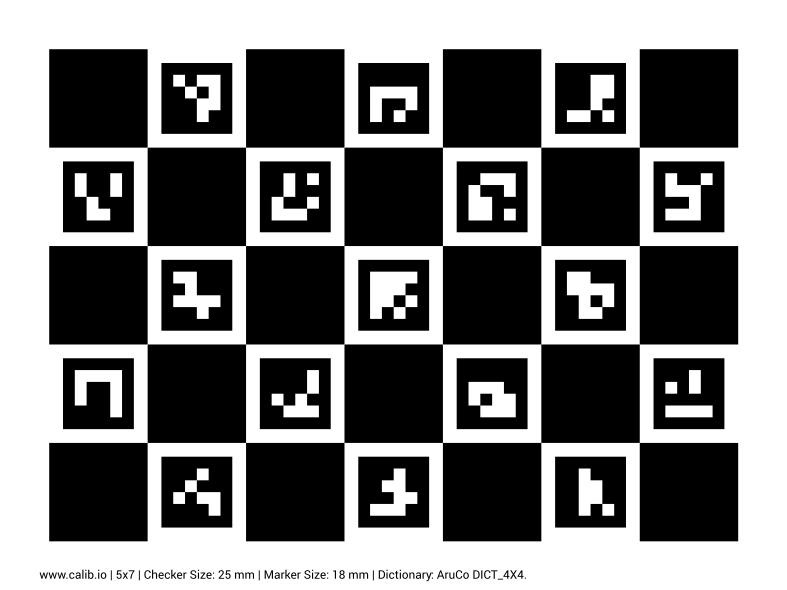
\includegraphics[width=0.7\textwidth]{figs/calib_io_charuco_200x150_5x7_25_18_DICT_4X4.png}
%       \caption{ArUco marker used to allow the segmentation for aligning the digital twin accordingly to the real environment}
%       \label{f:aruco_marker}
%       \end{subfigure}
%         \hfill % This command adds space between the subfigures
%       \begin{subfigure}[b]{0.45\textwidth}
%           \centering
%           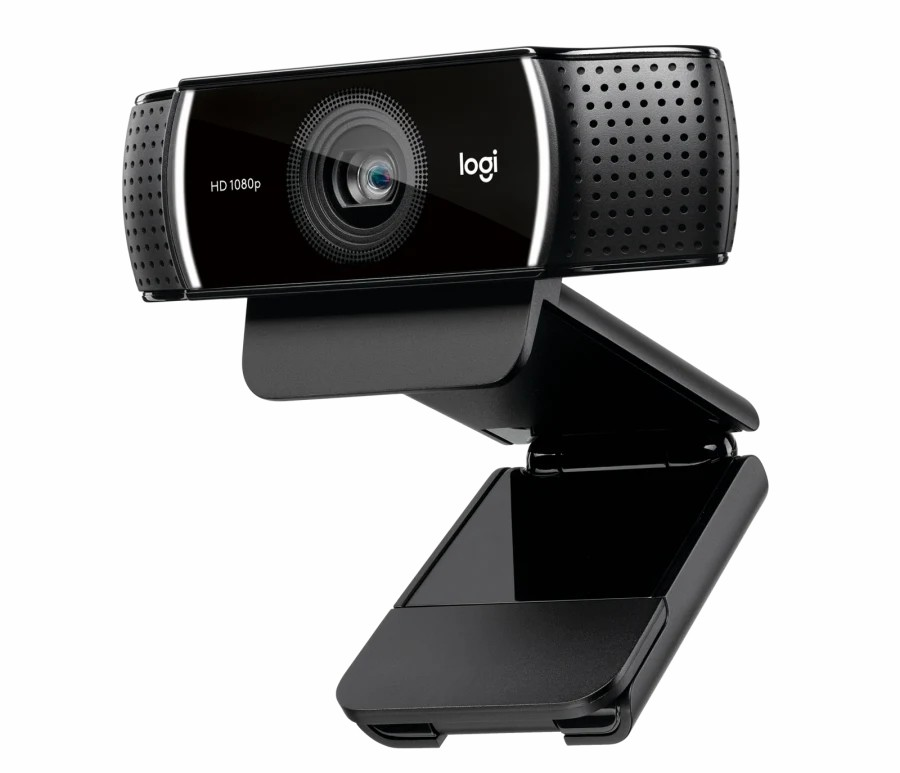
\includegraphics[width=0.7\linewidth]{figs/camera-c922.jpg}
%           \caption{Logitech c922 camera, used for testing on-site application developments}
%           \label{fig:camera-c922}
%       \end{subfigure}
%       \caption{ArUco marker used with the Logitech c922 camera for segmentation and manipulation of virtual environment}
%   \label{marker-camera}
%   \end{figure}
  